
%%%%%%%%%%%% 1 %%%%%%%%%%%
\chapter{Introduction and Motivation}
		The universe is vast, surprising, and has still just begun to be explored by humanity.  As telescopes become larger and more sensitive, we as a species can peer further away from our tiny blue speck with increasing clarity.  However, the absorption and scattering of high energy photons in the interstellar medium clouds much of the energetic universe from our gaze.  Nevertheless, there is a constant flux of hadronic particles incident on earth from various cosmic accelerators which survive the attenuation over universe scale distances.  These messenger particles provide a new window into regions of the universe that were previously inaccessible, and their observation remains a frontier in astrophysics.
%%%%%%%%%%%%%%%%%%%%%%%
\section{Cosmological Theory}
	\subsection{Cosmic Ray Detection History}
	Cosmic Rays (CRs) were first observed over a century ago, when an unexpected increase in ionizing radiation was observed as altitude increased (Figure \ref{fig:HessKol}).  Previously, it was expected that terrestrially measured radiation was caused by radioactive element decays within the earth's crust, however this additional radiative component was indicative of a source far from the Earth~\cite{HessCosmicRay}.  This discovery spawned a search for the sources of these particles raining down from the heavens.  In the subsequent hundred years, hundreds of experiments have taken up the task of measuring and characterizing cosmic rays incident on the earth, utilizing a variety of techniques~\cite{Olive:2016xmw}.  However, the search for cosmic accelerators able to produce the highest energy cosmic rays that have been experimentally measured remains an unsolved problem in physics that persists to the present day. 
	
\begin{figure}
\centering
	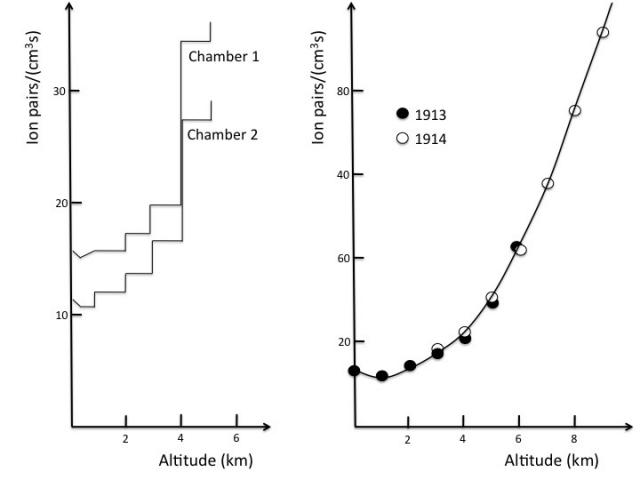
\includegraphics[width=0.7\textwidth]{figures/HessKol}
	\caption{Measurements of increasing ionizing radiation as a function of energy, by Hess in 1912 (left) and Kolhörster in 1913 (right), which provided strong evidence for an extra-terrestrial particle flux~\cite{HessKolPic}. }
\label{fig:HessKol}
\end{figure}
	
	\subsection{Cosmic Ray Physics and Cosmology}
	While the sources of cosmic rays remain unknown, their nature opens up the doors to many novel measurements of cosmological phenomenon that occur at extreme distances and energies.  Much of the universe is opaque to the traditional astronomical messenger particle, the photon, at high energies.  High energy gamma rays undergo electron-positron pair production in the presence of a magnetic field, effectively halting their travel before they can reach Earth.(Figure \ref{fig:observableUniverse}~\cite{RevModPhys.41.581}).  Additionally, the exceptionally high energies of particles detected by cosmic ray observatories, on the order of $10^{20}$~eV, dwarf the energies produced at terrestrial particle accelerators.  These particles can shed light on the world in the ultra high energy (UHE) regime.

\begin{figure}
\centering
	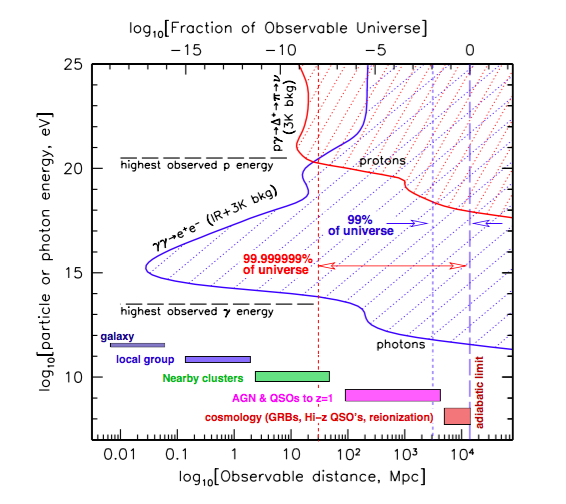
\includegraphics[width=\textwidth]{figures/ObservableUniverse}
	\caption{Interaction distances for photons and protons.  Shaded regions represent regions of the universe which are opaque to an astronomical particle. Plot courtesy of Dr. Peter Gorham.}
\label{fig:observableUniverse}
\end{figure}
	
	The observed energy spectrum of these hadronic particles introduced additional puzzles. As energy increases, the number of candidate sources for cosmic rays diminishes, leaving few to no candidates within our galaxy~\cite{RevModPhys.71.S33}.  Flux density as a function of energy, shown in Figure \ref{fig:cosmicrayflux} is well measured up to the EeV energy scale with modern experiments, however in the UHE region, those particles with energies above $10^{18}$eV, statistical limitations caused by the incredibly low flux, on the order of \SI{1}{\km^{-2} century^{-1}}, prevent accurate pointing to source locations.  Additional measurements are required to determine the transition between CRs emanating from galactic and extra-galactic sources.

	Using cosmic rays as astronomical messenger particles presents new difficulties as well.  At lower energies, traveling charged particles will have their courses bent by the Lorentz force while transiting the magnetic fields of stellar objects. Subsequently, inverting their incoming detection vector will no longer yield accurate pointing back to the source accelerator.  This is depicted in Figure \ref{fig:CosmicRayDeviation}.  Higher energy cosmic rays are proportionally less effected by magnetic fields due to their increased rigidity, and chargeless particles do not suffer this effect at all.  This increases the desirability of detectors that can measure messenger particles with a low flux or a small cross section.
	
	The composition of cosmic rays at the highest energies remains under investigation as well.  An extensive air shower produced from a CR interacting with an atmospheric molecule has identical secondary detection characteristics whether the initial source particle was heavy ions or protons.  However, acceleration mechanisms and evolution models for various compositions vary wildly, impacting cosmic evolution and the resulting cosmic ray flux models~\cite{UHECRcomposition}.  Recent measurements studying the maximum shower depth of air showers suggests a mixed composition, and possibly a hint at a transition from galactic to extragalactic source accelerator at EeV energies~\cite{AugerXmax}\cite{AugerXmaxDiscussion}. Additional experimental observations of these cosmological particles will yield a better understanding of both the structure of matter and energy within the universe at large, as well as fundamental physics processes energetically unachievable from existing collider experiments. The creation and propagation of Ultra High Energy Cosmic Rays (UHECRs) through the universe opens a window to understanding of extreme high energy physics.
	%Do the actual math for converting center of momentum energy to relativistically shifted energy, because though UHE is 6 orders of magnitude above CERN at TeV energies, CERN's two colliding TeV beams only end up like 100x below.
	
	
	%%From the July 24th ANITA phone call about ICRC and a good discussion about it.  Takeaway: no one knows composition
	%Most recently, Iron ions have been excluded by Auger and TA, with evidence pointing to proton or mixed composition at the highest energies.\cite{ICRC2017}  The key parameter is the maximum energy of the proton, so any other composition, (CNO, carbon/nitrogen/oxygen) would suppress the neutrino flux as ion mass increases.  Additionally, observed cosmic ray composition at earth is not necessarily representative of the high energy acceleration environment at redshifts of two or three.  Charge to mass ratio is also important.

		
\noindent
\begin{figure}
\centering
	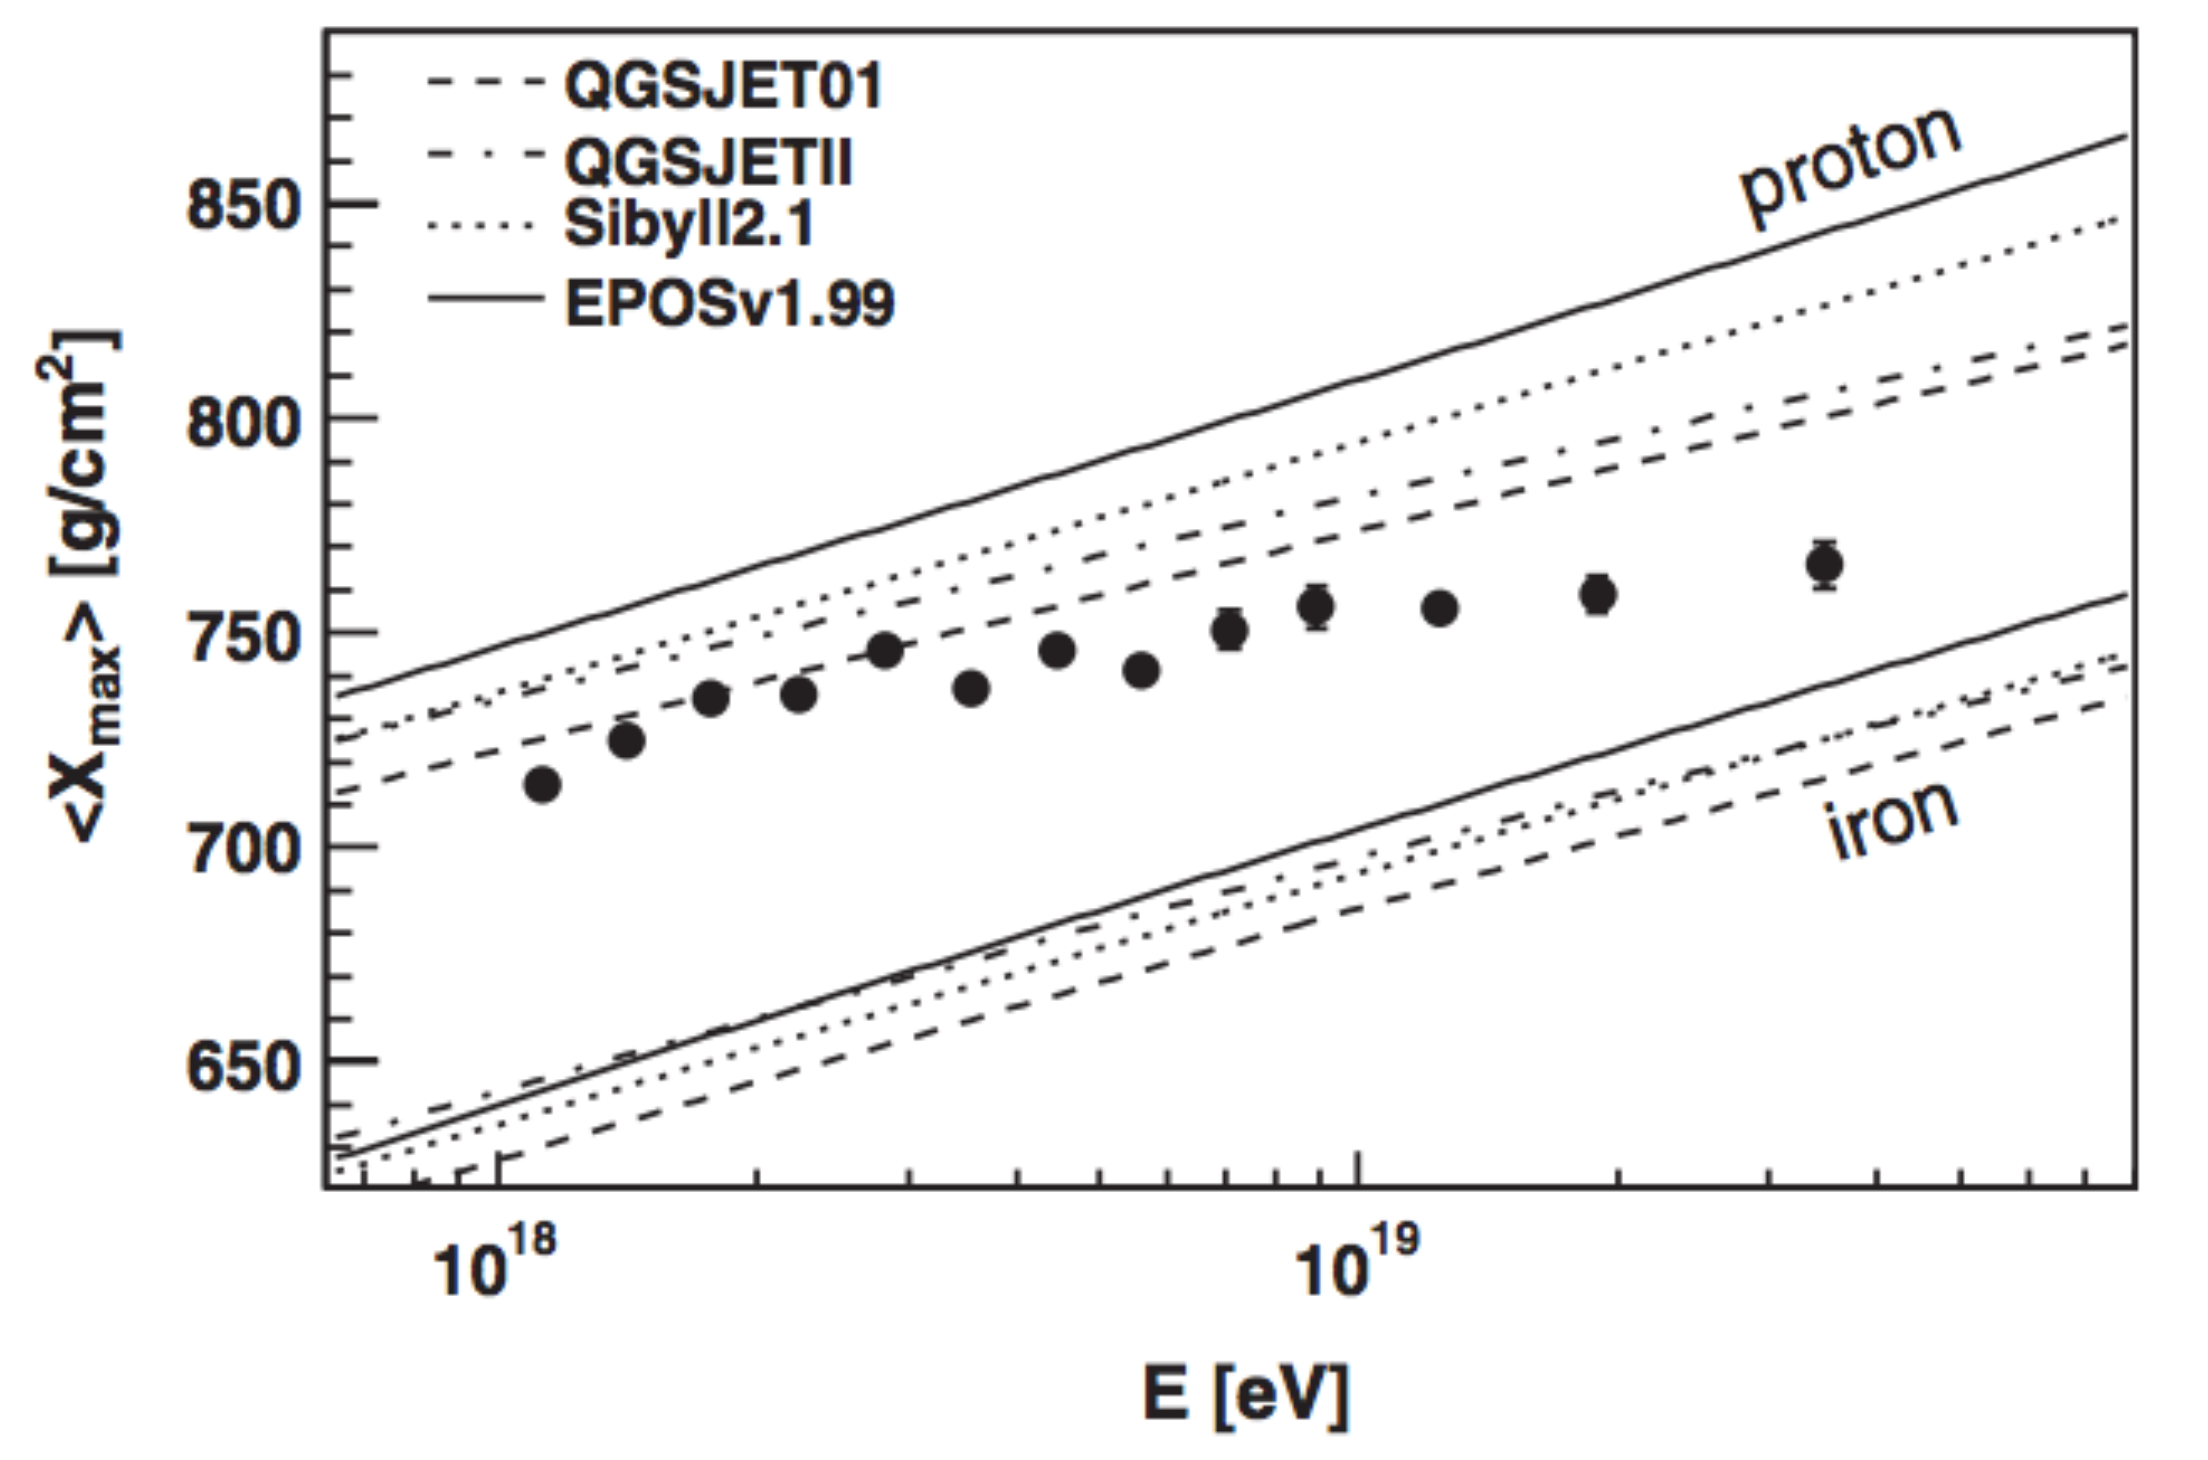
\includegraphics[width=\textwidth]{figures/AugerXmax}
	\caption{Measurements of cosmic ray maximum shower depth by the Auger observatory.  Modeled lines show theoretical predictions for two cosmic ray compositions, iron and protons\cite{AugerXmax}}
	\label{fig:AugerXmax}
\end{figure}

\noindent		
\begin{figure}
	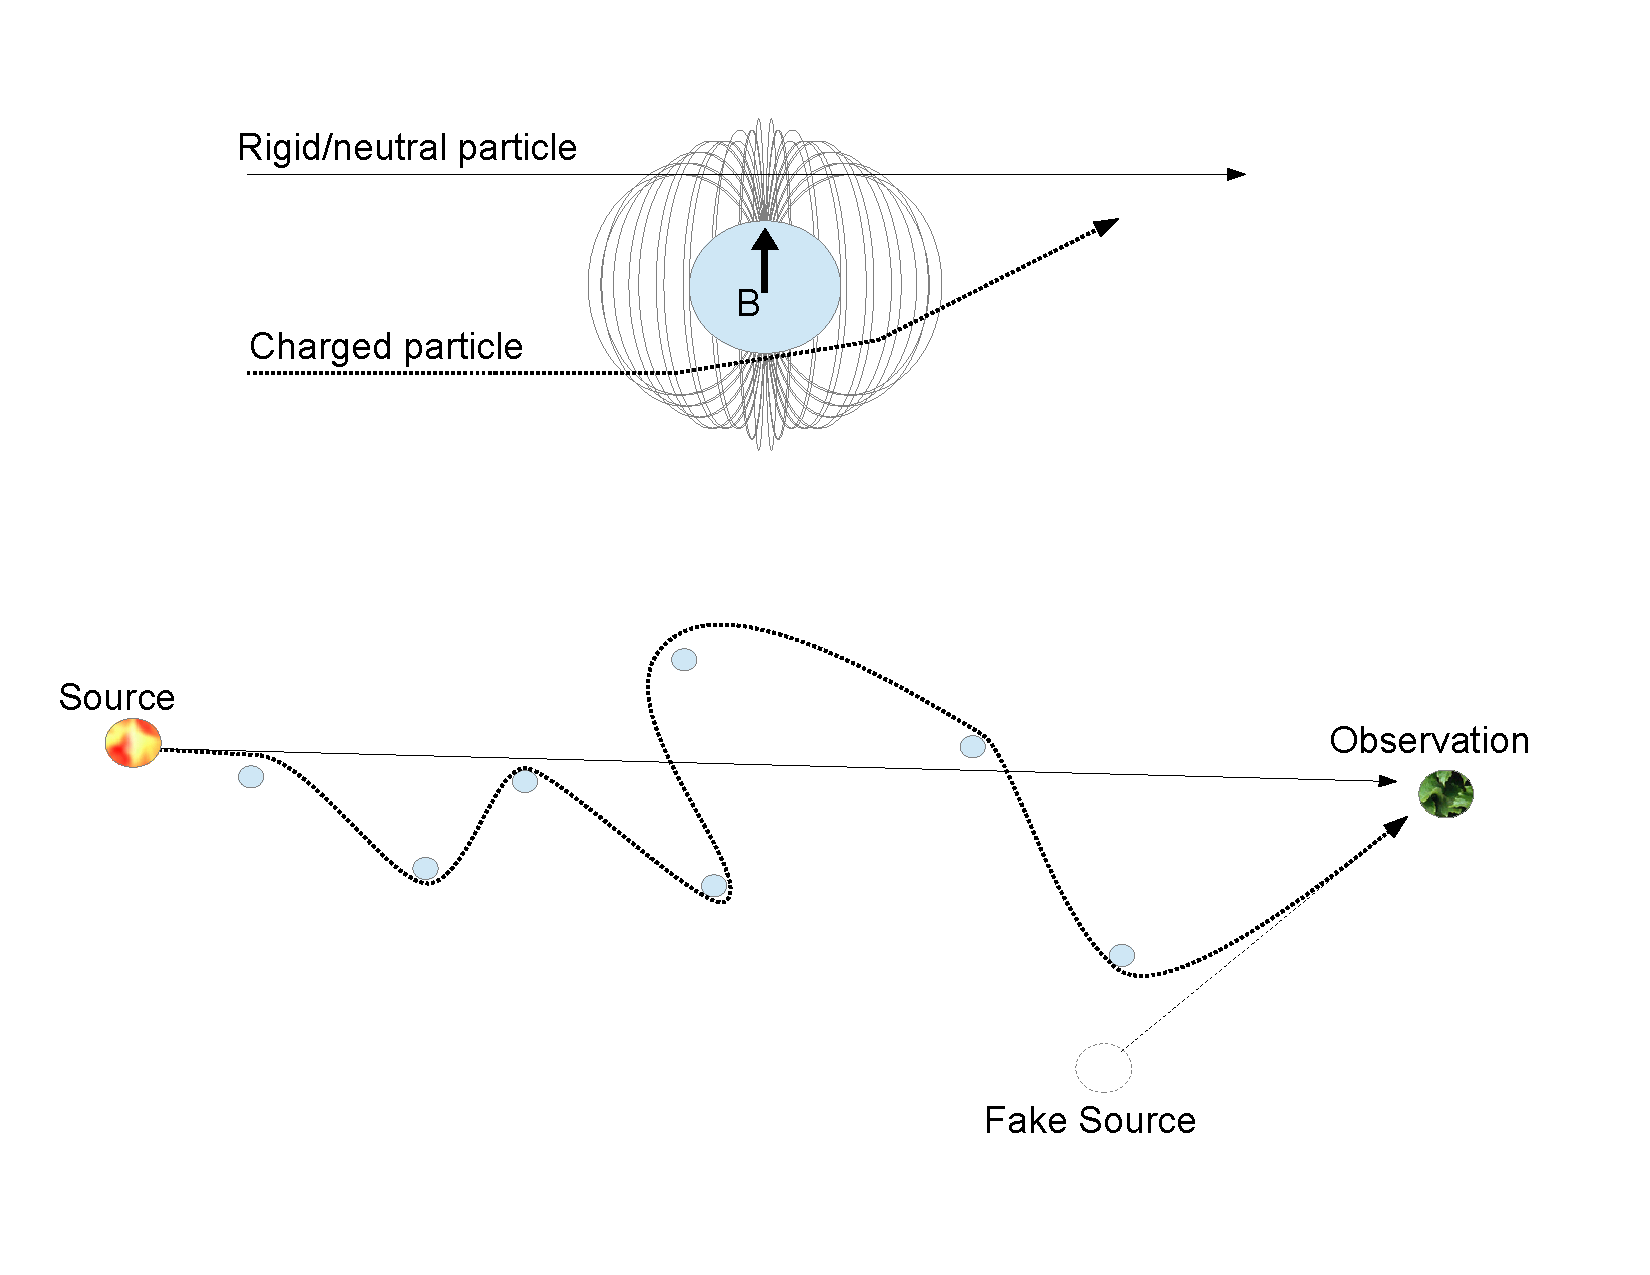
\includegraphics[width=\textwidth]{figures/CosmicRayDeflection}
	\caption{Top: A simplified diagram of lorentz-force induced curvature in low energy cosmic rays.  Bottom: An example of why magnetic deflection distorts the observed CR source location}
	\label{fig:CosmicRayDeviation}
\end{figure}
		

\noindent		
%\begin{wrapfigure}{L}{0.5\textwidth}
\begin{figure}
	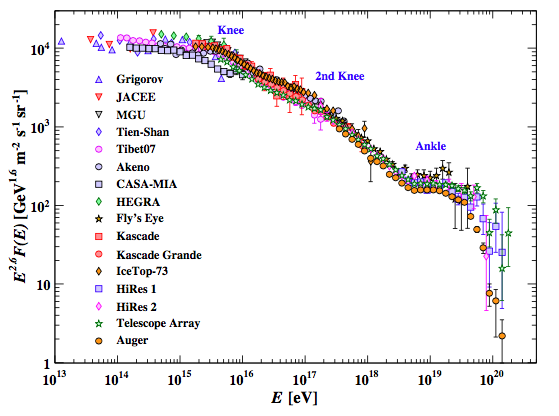
\includegraphics[width=\textwidth]{figures/CosmicRayFluxMeasurements}
	\caption{The all-particle spectrum as a function of energy-per-nucleus from measurements\cite{Olive:2016xmw}}
	\label{fig:cosmicrayflux}
\end{figure}
%\end{wrapfigure}		
		


\section{Neutrino astrophysics and the GZK interaction}
		The steep decline in observed flux measured by detectors alludes to an interaction mechanism that opens up a new detection prospect for UHE Cosmic Rays.  A sharp decrease in energy flux spectrum at 10$^{19}$~eV Figure \ref{fig:cosmicrayflux}, the sharp decrease at 10$^{19}$eV corresponds to an interaction of a rest proton with a high energy gamma ray through a delta resonance.  Shifting the frame of reference to a relativistic proton colliding with a low energy photon, one arrives at an accurate description of a cosmic ray transiting the cosmic microwave background (CMB) radiation that isotropically pervades the universe~\cite{WMAPCMBResults}.  This interaction was predicted by Greisen, Zatsepin and Kuzmin~\cite{GZK}, and represents a theoretical high energy limit on particles coming from outside of the galaxy.  Colloquially known as the GZK limit and present at 5x10$^{19}$ eV, particles with energies above this threshold will weakly scatter off the CMB and decline in energy through emission of secondary particles~\cite{GZK}.  Observatories measuring UHE cosmic rays have detected a decrease in the quantity of observed particles consistant with a GZK induced suppression~\cite{GZKMeasurement}. Cosmic ray particles have also been observed exceeding this limit, suggesting an additional unknown source within the galaxy.  The low statistics of particles observed at this energy prevent identification of a specific source.  Since particles are present at these high energies, it would also be expected that other regions of the universe also contain accelerators capable of creating cosmic rays in excess of the GZK limit, thus motivating a UHE neutrino flux.
		
		The GZK process has multiple channels, each of which produce an ultra high energy neutrino (UHE$\nu$) messenger particle that could subsequently be detected on earth (Figure \ref{fig:GZKDiagram}~\cite{GZK}). The cross section of neutrinos has been measured in accelerator facilities to be vanishingly small at modern accelerator scale energies~\cite{neutrinoCrossSectionMeasurements}.  However, at energies out of reach of modern accelerators, cosmic accelerators could illuminate our understanding of neutrino cross section.  The neutrino cross section at energies above those measured by accelerator facilities has been estimated by using standard model particle physics~\cite{neutrinoCrossSectionExtrapolation}. This small cross section allows the GZK interaction messenger neutrino to traverse unimpeded through the intergalactic medium before subsequently interacting with earth.  Additionally, the uncharged nature of neutrinos allow them to travel in a straight line from their source locations without Lorentz deflection from intervening magnetic fields.  Neutrinos have an extremely small cross section, such that their mean free path length through the universe is essentially infinite. Experiments with the capability to detect these particles will allow an unparalleled view into the depths of the cosmos.

\noindent		
%\begin{wrapfigure}{L}{0.5\textwidth}
\begin{figure}
	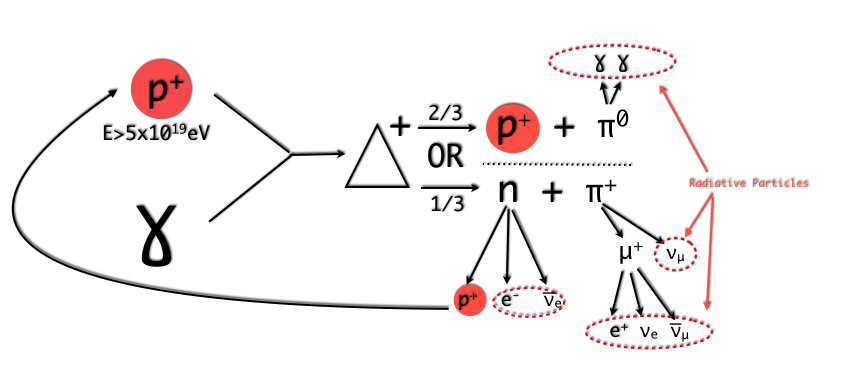
\includegraphics[width=\textwidth]{figures/GZKDiagram}
	\caption{A diagram of the possible resultant particles of a GZK interaction between a photon and the CMB.}
	\label{fig:GZKDiagram}
\end{figure}
%\end{wrapfigure}		
			
		
	\subsection{Unexplained UHE Source Mystery}
		Though there are numerous low to mid-scale energy cosmic ray sources that have strong theoretical motivation and experimental evidence, above 10$^{17.5}$~eV the number of candidates becomes constrained and extra-galactic source hypotheses are required. \cite{RevModPhys.71.S33}  Due to the higher flux of nearby low energy cosmic ray sources, many experiments have gathered evidence to support source candidates within our galaxy as accelerators.  However, above the GZK suppression limit there remains little collected experimental evidence that describes the transition to extra-galactic sources. These higher energy objects include such objects and Active Galactic Nuclei (AGN), supernova, quasars, gamma-ray bursts, as seen in Figure \ref{fig:cosmicAccels}  However, the small statistics afforded by incident particles at the UHE end of the spectrum makes identifying their acceleration mechanisms much more difficult, and requiring extremely voluminous detectors.

\begin{figure}
	\centering
	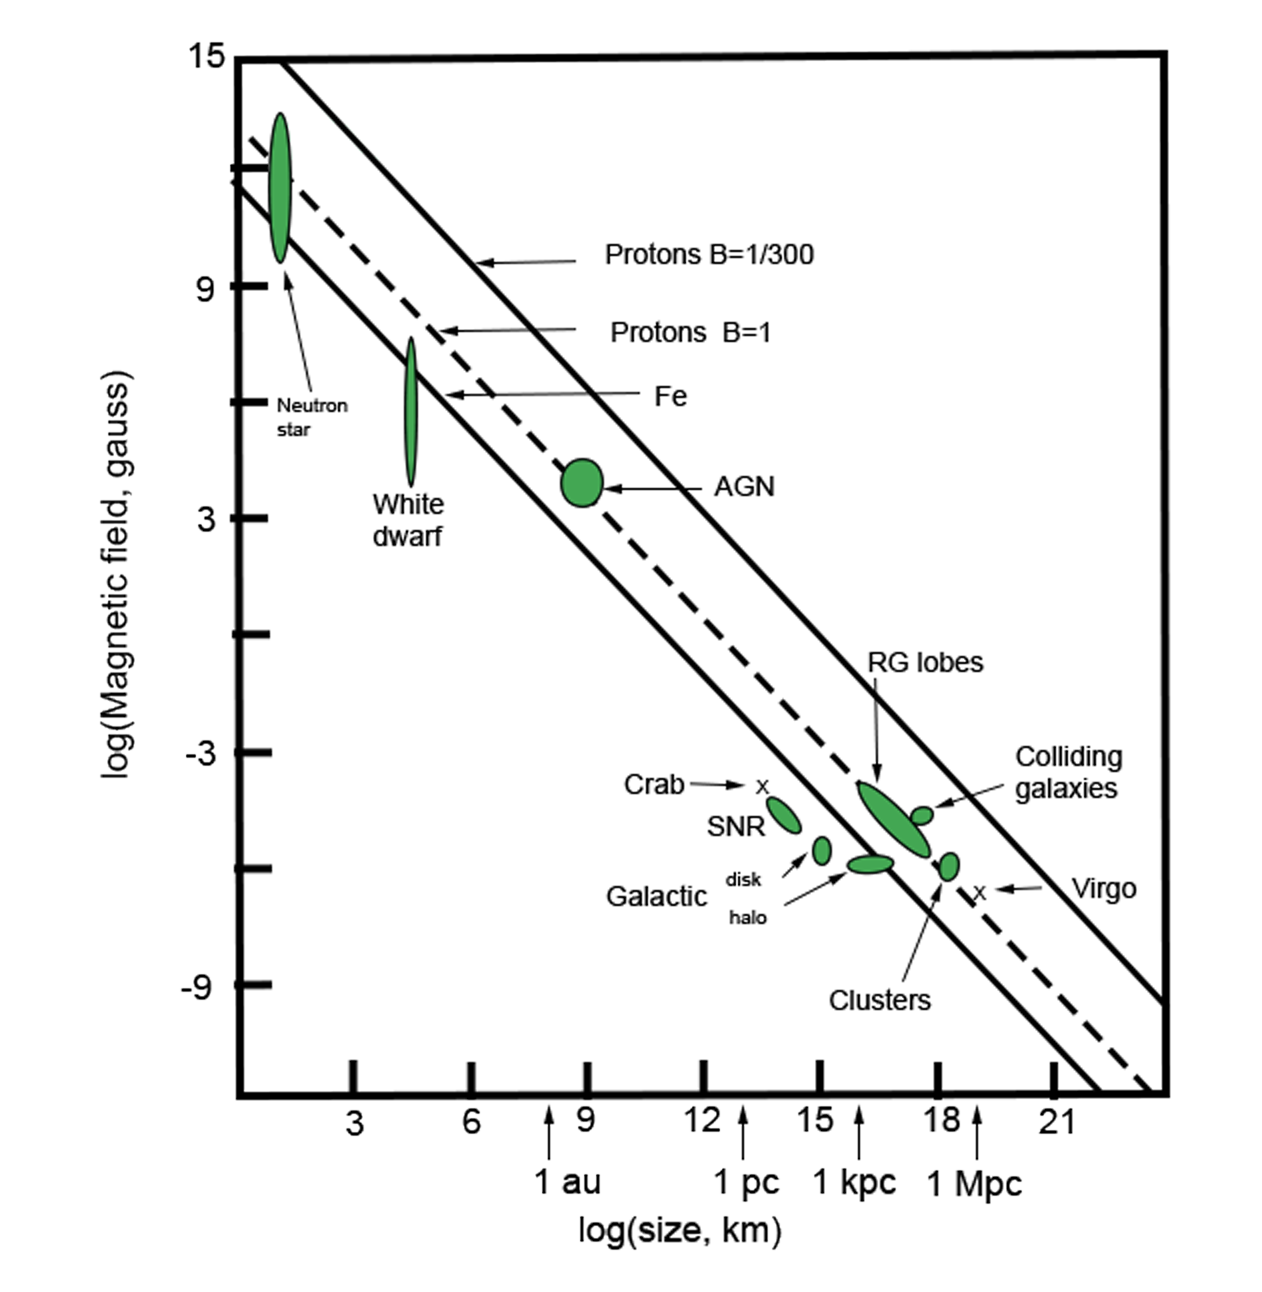
\includegraphics[width=\textwidth]{figures/cosmicAccelerators_trace}
	\caption{Theorized cosmic accelerators plotted by their size and peak magnetic field.  The dashed line denotes a field strength capable of accelerating protons to $10^{18}$ eV. Plot vectorized from~\cite{RevModPhys.71.S33}. }
	\label{fig:cosmicAccels}
\end{figure}


\section{Neutrino Detection on Earth}
	The neutrinos produced in GZK interactions are messenger particles that carry information about UHECRs produced outside the galaxy to earth at energies above the GZK suppression effect.  Astronomical neutrino telescope observations have been carried out at lower energies since the discovery of the particle itself~\cite{Homestake}. Recently however, there has been a notable increase in detector scale and energy sensitivity.  The term ``cosmic ray'' describes any high energy particle incident on earth (including gamma rays) and thus, for the purposes of this dissertation, neutrinos fit the description of cosmic rays.
	
	The largest notable difference between observations of UHE neutrinos and cosmic rays is the medium in which they are most likely to interact.  While cosmic rays have large cross sections and are predicted to interact with even low density media, neutrinos require a medium with far higher density.  The primary observation location for cosmic rays is thus within the atmosphere, while neutrinos are generally observed in custom-constructed and instrumented media.  Both particle interaction lengths can be described by the traversed density, or specifically for the case of cosmic rays the atmospheric depth, units of \SI{}{\gram\per\square\centi\meter}.  For UHE$\nu$s however, this term becomes larger than the integrated total density of the atmosphere regardless of incoming slant angle.  The neutrino will therefore either skim the atmosphere entirely if shallow enough, or interact within the earth if too steep.  However, if a dense dielectric solid is introduced or utilized at the Earth's surface by an opportunistic experimenter, it is possible to capture neutrino interactions within the field of view of detection equipment.  This equiptment can capture the induced electromagnetic showers from a high energy particle shower.
	
	\subsection{Charged current and Neutral Current interactions} 
		Neutrinos have two distinct interaction classifications, Neutral Current (NC) and Charged Current (CC)~\cite{neutrinoCrossSectionMeasurements}.  Feynman diagrams depicting these interactions can be seen in Figure \ref{fig:NC_CC}.  Both interactions can occur with either baryons, such as protons and neutrons, or leptons, such as electrons.  The two interactions have differing cross sections and result in different resulting particles with a large fraction of the incident energy.  These different processes will both affect the initial UHE particle propagation, but only the CC interaction will produce a detectable signal.
	
\begin{figure}
	\centering
	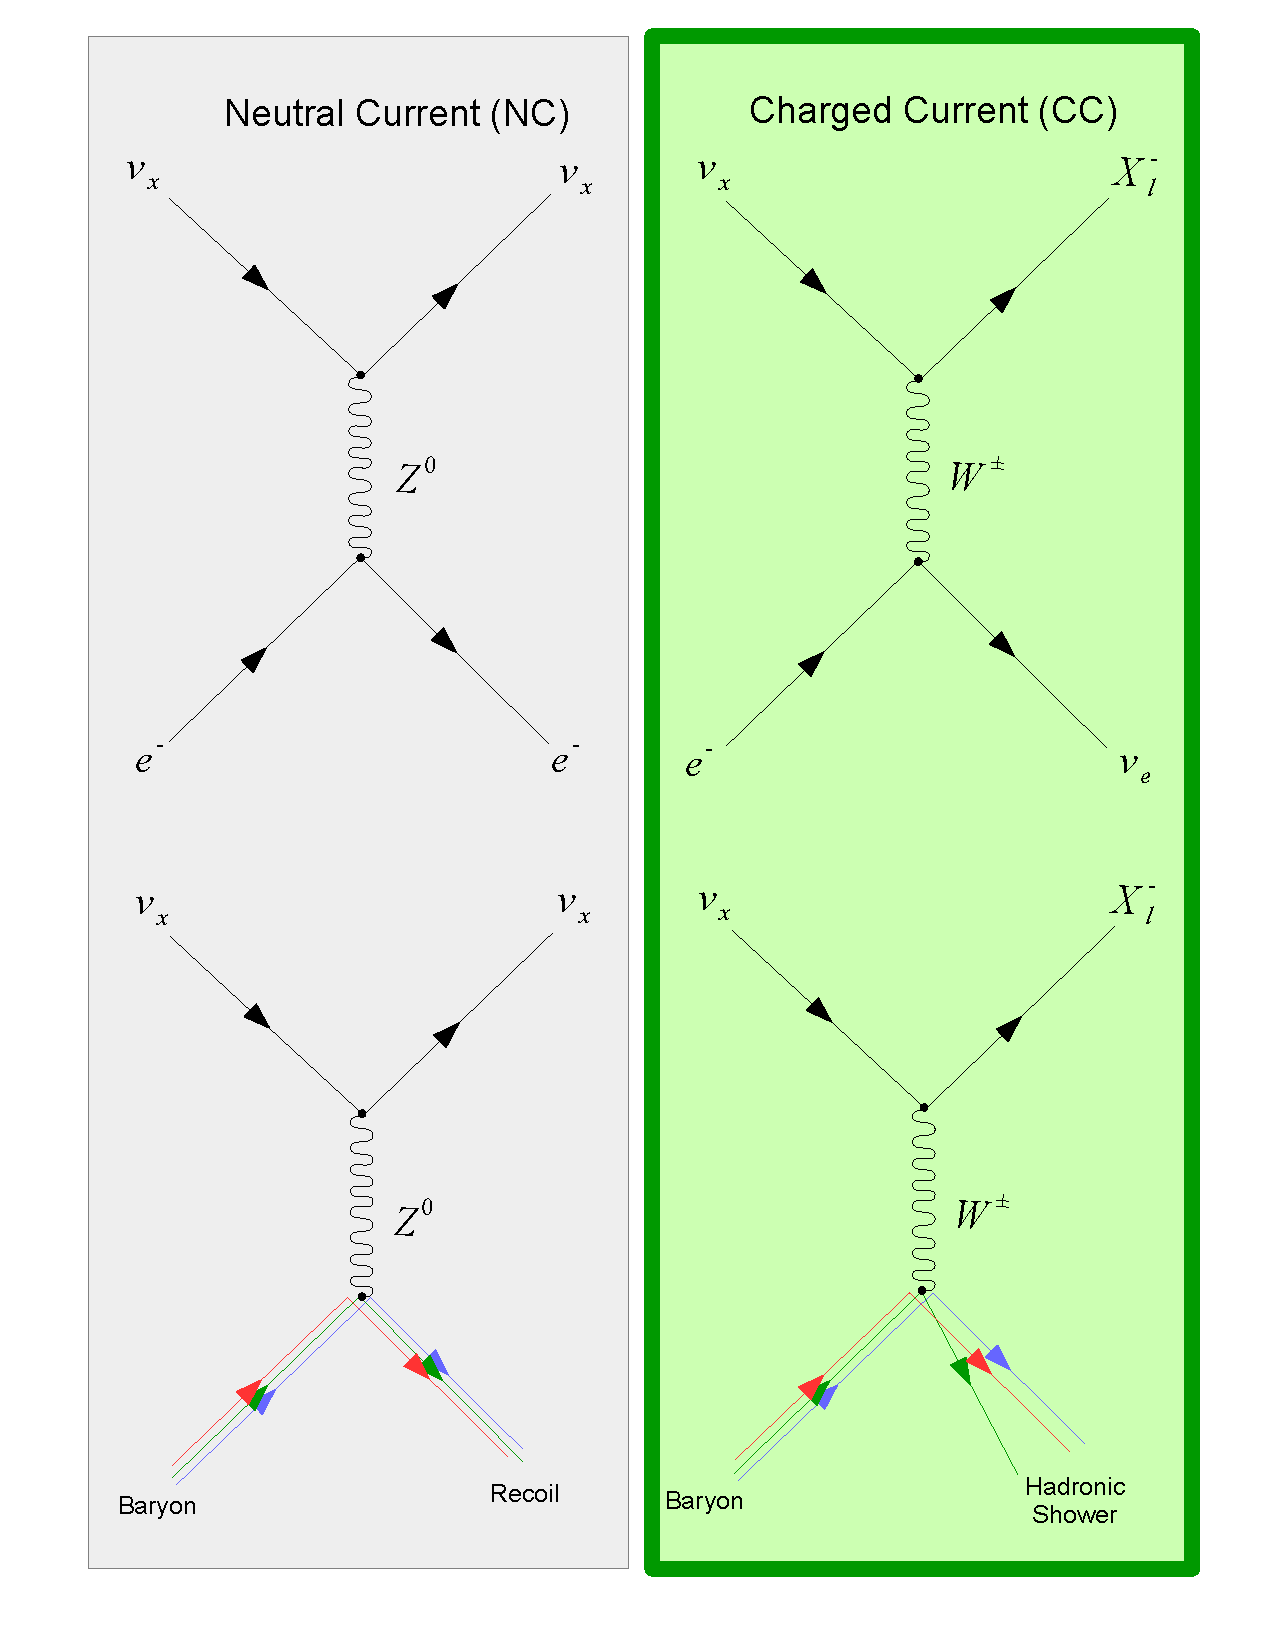
\includegraphics[width=0.85\textwidth]{figures/NC_CC}
	\caption{Feynman diagrams showing neutrino interactions.  The weak force boson mediating the interaction defines whether an interaction is charged current ($W^{\pm}$) or neutral current ($Z^{0}$).  Neutral current interactions do not result in secondary showers that produce detectable electromagnetic radiation.  Charged current interactions, marked in green, can produce extensive showers with and electromagnetic component detectable by instruments.  $X^{-}_{l}$ denotes a charged lepton with the flavor of the incident neutrino $\nu_{x}$.}
	\label{fig:NC_CC}
\end{figure}

	
		A neutral current interaction occurs through the exchange of a $Z^{0}$ boson, and transfers a fraction of its energy and momentum to the particle with which it interacted.  The resulting particles from the interaction are the same as the initial particles, with the incident neutrino retaining a majority of the momentum.  Incident UHE neutrinos can "skip like a stone" off the dense matter of the earth, continuing to propagate, with much of their initial energy, through the earth.  The resulting energy transfered to the opposing particle is insufficient to cause a detectable radiative shower.
		
		A charged current interaction involves the exchange of a $W^{\pm}$ boson, and results in the neutrino being converted into a similarly flavored and charged lepton.  The charged lepton, which retains a large fraction of the energy from the incident UHE$\nu$ and has a much larger cross section, quickly proceeds to scatter again and spark a large shower of secondary particles.  The CC interaction produces a strong electromagnetic radiative signal that, if given a sufficiently transparent interaction medium, can be detected by physics instruments.
			

	\subsection{Extensive Air/Ice Showers}
		A highly energetic particle interacting with the hadronic matter present in Earth's atmosphere, or in any  dense material, creates an extended series of particle production, scatterings, and decays.  The extensive shower of particles scattered or created from a single high energy source particle has been appropriately dubbed an Extensive Air Shower (EAS).  These showers produce both traveling messenger particles that can be observed through weakly interacting secondary scatterings in instrumented transparent scintillating media, as well as through primary radiation, which is the topic of this thesis.  This primary radiation is stimulated by the appearance of moving charged particle pairs that travel along the principle shower axis.  There are two main electromagnetic radiative effects, detailed below and depicted in Figure \ref{fig:EASRadiation}, that can be observed in the  VHF (3MHz to 300MHz) and UHF (300MHz to 3GHz) bands of the electromagnetic spectrum.  This region of the spectrum has very good transmissive properties in the atmosphere, as well as within many dense solids.\cite{Besson2009348}\cite{VuFind-000215473}\cite{Barrella:2010vs}
		

\begin{figure}
	\centering
	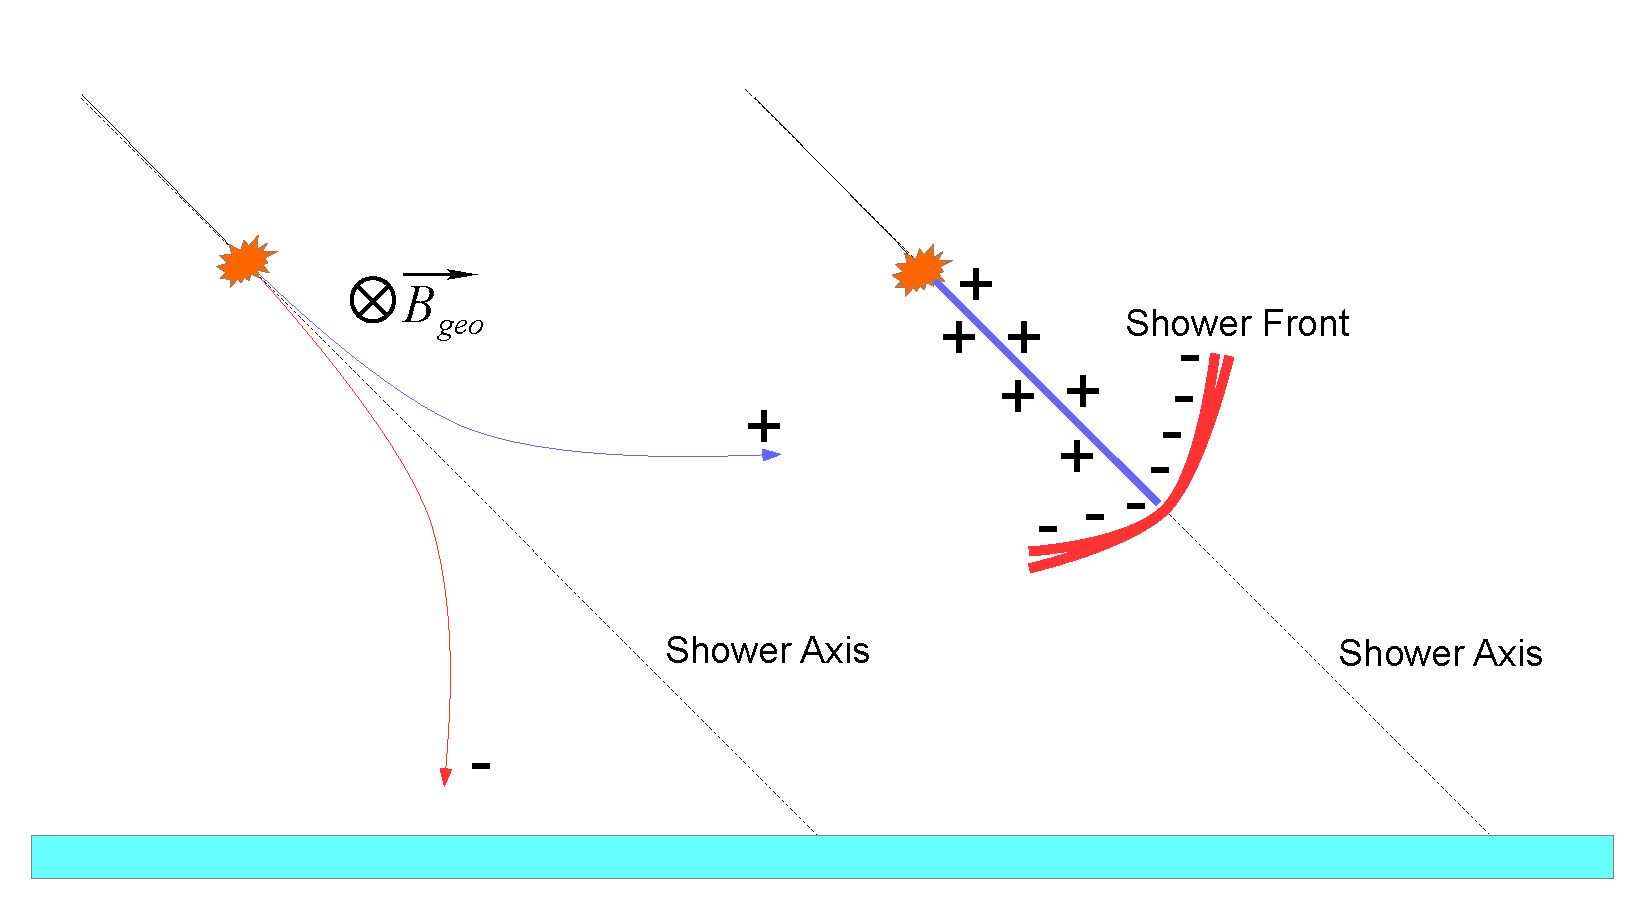
\includegraphics[width=\textwidth]{figures/EASRadiation}
	\caption{Simplified schematic of two EAS radiative trasmission mechanisms, geomagnetic (left) and charge-excess, or Askaryan, radiation (right)}
	\label{fig:EASRadiation}
\end{figure}

	
	\subsection{Geomagnetic Radiation}
		The primary and strongest radiative effect in an EAS is from a longitudinal charge separation created from a Lorentz deflection as the newly created grouping of charged particles move through the geomagnetic field of the Earth.  As the shower is required to have zero net charge (A CR will have a total incident charge of +1 and a neutrino has no charge), an equal number of positively and negatively charged particles are generated.  The Lorentz force, $F=q(\vec{E}+\vec{v}\times\vec{B})$, acting with opposite sign on oppositely charged particles, will inducing a spacial separation.  This dynamically varying charge separation emits radiation with a linear polarization orthogonal to both the magnetic field and the shower axis with an intensity proportional to the incoming shower energy and magnetic field.  This effect has recently been measured using an accelerator beam induced shower transiting an induced magnetic field.\cite{SLACT510}
	
	\subsection{Askaryan Effect}
		A secondary radiation component, theorized by Gurgen Askaryan in 1962, is a build up of negative charge at the front of the shower core as electrons are created and scattered forward, while their positron pairs are annihilated.\cite{Askaryan:1962hbi}  This creates a charge separation between the negatively charged shower front and the positively charged shower path.  This relativistic velocity charge buildup will radiate coherently at critical off-angles where the wavefronts constructively interfere.  This is visible in the time domain as a sharp, broad spectrum impulse,  as the stationary viewer observes an enormous instantaneous charge flux, as seen in Figure \ref{fig:Cherenkov}~\cite{PhysRevD.84.103003}.  This effect has much more recently been measured at particle accelerators in a variety of materials, including ice,\cite{PhysRevLett.99.171101} salt~\cite{PhysRevD.72.023002}, and silica sand~\cite{PhysRevLett.86.2802}.  An example accelerator initiated Askaryan pulse in ice measured by the ANITA electronics is visible in Figure \ref{fig:ANITASLACPulse}.
		
		
\begin{figure}
\centering
	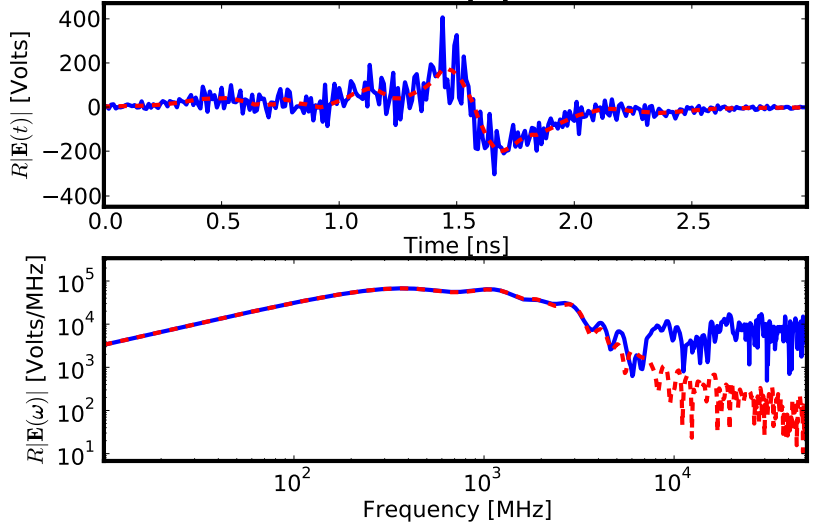
\includegraphics[width=\textwidth]{figures/AskaryanSimulation}
	\caption{The electric field of an Askaryan pulse observed close to the critical angle in the far field generated by a mathematical model(red), and with the ZHS simulation package(blue) \cite{PhysRevD.84.103003} }
	\label{fig:AskaryanSimulation}
\end{figure}

\begin{figure}
\centering
	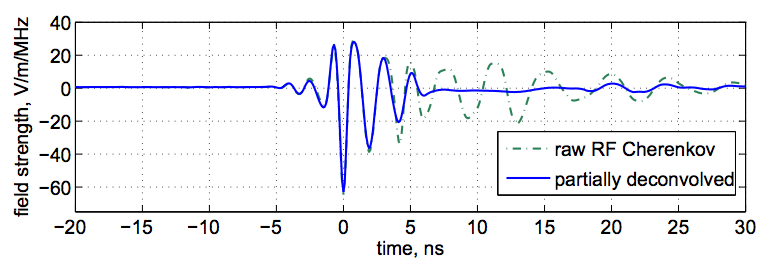
\includegraphics[width=\textwidth]{figures/ANITASLACImpulse}
	\caption{An example accelerator initiated Askaryan pulse in ice measured by the ANITA electronics  The dispersion in the signal is introduced by the band-pass filtering in the RF signal chain\cite{PhysRevLett.99.171101} }
	\label{fig:ANITASLACPulse}
\end{figure}


\begin{figure}
\centering
	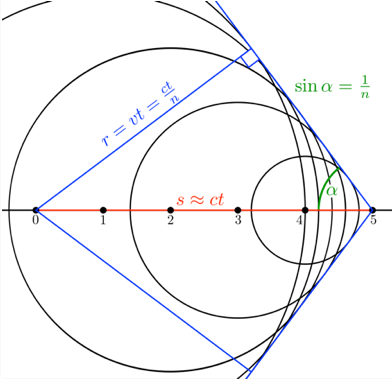
\includegraphics[width=0.5\textwidth]{figures/Cherenkov}
	\caption{An example diagram of the Cherenkov critical angle where the radiative components of a CR shower experience a signal boost.}
	\label{fig:Cherenkov}
\end{figure}


%	\subsection{Cherenkov Radiation}
%		Considering a realistic index of refraction for the dielectric medium in which a particle shower occurs results in a boost to both primary sources of shower radiation at distances slightly off the shower axis.  This is caused by constructive interference induced by the relativistically propagating shower through a dielectric, in which light propagates at $<c$, at a critical off angle, which corresponds with Cherenkov radiation.  This process is shown in Figure 
		



	\subsection{Tau-\texorpdfstring{$\nu$} Specific Detection Prospects}
		Though the Earth becomes opaque to neutrinos at high energies, secondary particles may have a higher mean free path, which can widen the field of view past the narrow sliver of ice at the horizons.  A Tau lepton ($\tau$), produced from a similarly flavored neutrino undergoing a charged-current interaction, have an extremely short lifetime, 2.9e$^{-13}$~s, and can leptonically decay back into a tau neutrino ($\nu_{tau}$) which can then continue to propagate.   The expected flavor production ratio from typical sources is expected to be $\Phi_{\nu_{e}}$ : $\Phi_{\nu_{\mu}}$ : $\Phi_{\nu_{\tau}}$ = 2:1:0, with few to no produced $\nu_{\tau}$ messenger particles.  Due to flavor mixing however, the cosmologically long distances traversed by a UHE$\nu$ is expected to provide an even distribution fraction of each flavor for detection at earth, $\Phi_{\nu_{e}}$ : $\Phi_{\nu_{\mu}}$ : $\Phi_{\nu_{\tau}}$ = 1:1:1.  
		
		This adds an additional propagation channel to be combined with the probability that the neutrino undergoes a NC interaction, decreasing a catastrophic decay (and resulting electromagnetic pulse) of the incident UHE$\nu$.  Taus decay hadronically 67\% of the time, where the majority of the tau energy is then carried away in the form of pions.  The remaining third of the time however the tau decays leptonically, producing a tau neutrino with a large fraction of the initial incident UHE energy.  Repeated regenerations of a UHE$\nu_{tau}$ will increase the propagation length of the initial particle, dramatically extending its travel distance through the earth~\cite{TauRegeneration}  The particle can then undergo a hadronic decay in the atmosphere, initiating an EAS that travels upwards from the surface of the Earth.  A diagram of the proposed, increased lifetime, UHE$\nu_{\tau}$ interaction timeline resulting in a detectable radio frequency electromagnetic signature is shown in Figure \ref{fig:TauRegeneration}.
		
\begin{figure}
\centering
	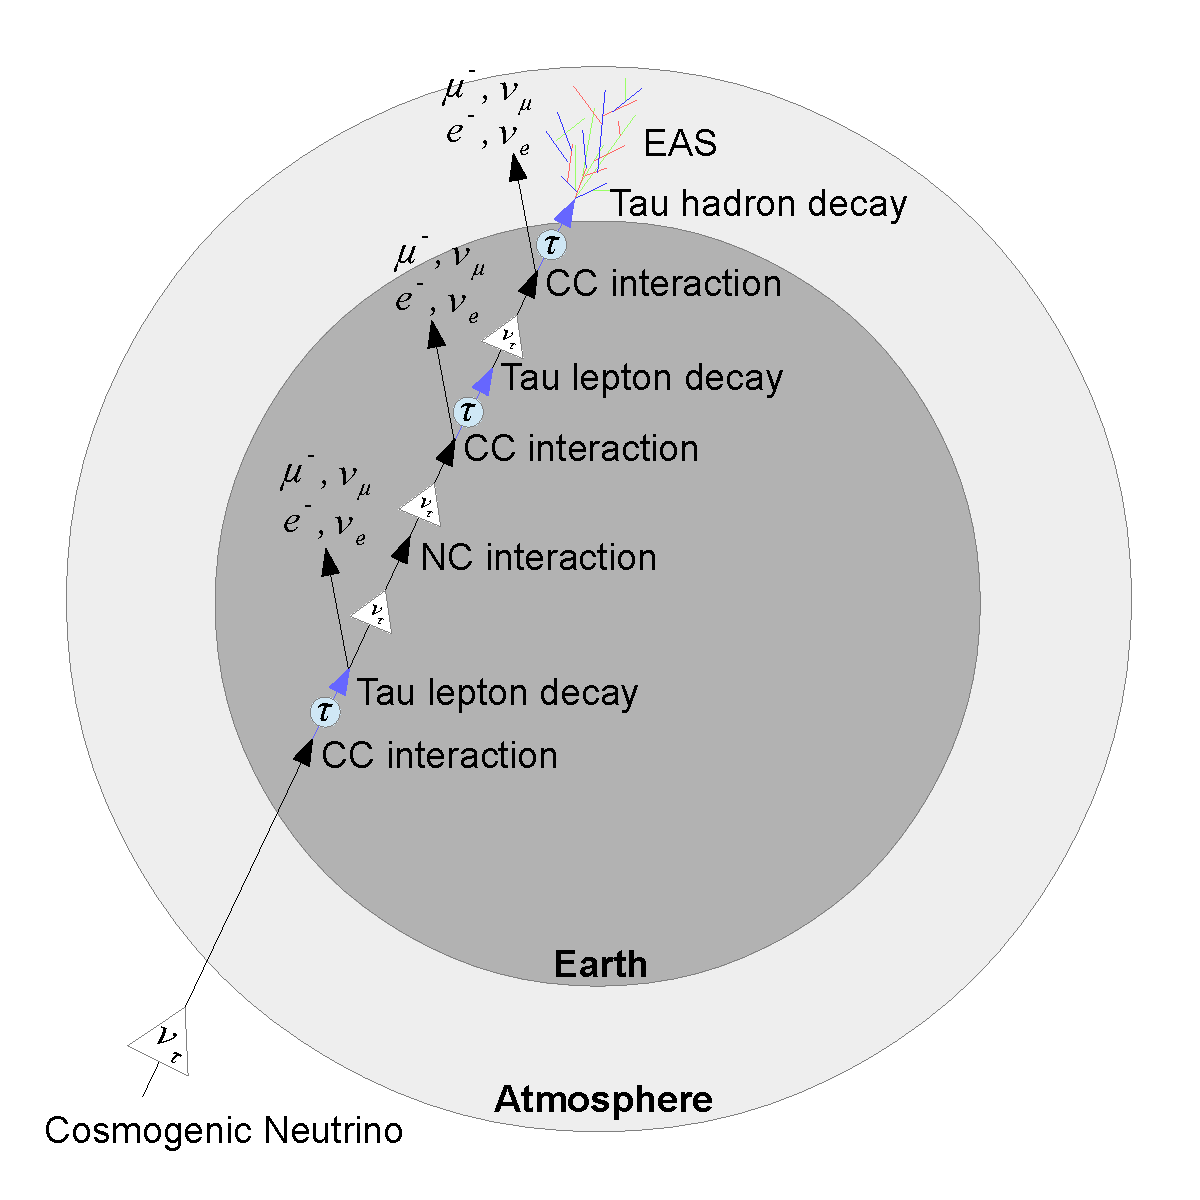
\includegraphics[width=\textwidth]{figures/TauRegeneration}
	\caption{An example of an incident  UHE$\nu_{\tau}$ undergoing multiple scatters within the earth before finally starting a detectable EAS in the atmosphere.  This type of interaction timeline is proposed as a detectable steeply up-going electromagnetic signature.  Figure not to scale.}
	\label{fig:TauRegeneration}
\end{figure}
		
		A UHE$\nu_{\tau}$ will thus behave characteristically similar to a UHECR, except that it will have a flipped polarity to a reflected down-going EAS, and a matched polarity to a directly viewed EAS.  Detection of UHE$\nu_{\tau}$s with this type of interaction history has recently been attempted by other experiments~\cite{AugerTauSearch}, though no events were identified.  A search for UHE$\nu_{\tau}$ particles was recently done for the ANITA1 data set as well, with one candidate found~\cite{PhysRevD.86.022005}.  ANITA has a unique opportunity to make observations of this type of regeneration 

\section{ANITA}
	Up to this point, I have mainly motivated a detectable physics hypothesis from established theories and measurements.  From here, I can introduce a detection platform for these physics phenomenon, the ANtarctic Impulsive Transient Antenna (ANITA).  EASs present in the atmosphere or in the dense, radio transparent, dielectric solid ice sheet covering the souther continent of Antarctica will produce unique and characteristic signals through the above particle interactions and radiative effects.  A high altitude, long duration, telescope platform would have an extremely large field of view, thus increasing the possibility of observing one of these rate interactions.  Additionally, downwardly moving atmospheric CR shower events can be both observed by the payload directly, or as reflections off the ice that covers the Antarctic continent.  These reflected pulses will have an inverted phase from the theoretical models of an EAS.  The following chapters detail the instrument, analysis, and simulation of the third ANITA flight.




